%% Estructura principal para un reporte de Trabajos intersemanales CIRCAE %%
%% Autor: Edison Abado Ancco

\documentclass[a4paper]{article} %tamaño del papel y el tipo de transcripción que será IEEE
\usepackage[margin=2.8cm]{geometry}
%\usepackage[total={6.5in,10in},left=1in,top=0.5in,includehead,includefoot]{geometry}
\usepackage[utf8]{inputenc} %el tipo de codificación que incluye símbolos como la tilde
\usepackage[spanish]{babel} % hacemos que nuestro documentación vaya en español
\usepackage{cite} % citas bibliográficas
\usepackage{graphicx} %gráficos, usaremos solo .jpg o .png con estándares que ya veremos
%\usepackage{subfigure} %usar subfiguras
\usepackage{url} %agregar direcciones url
\usepackage{amsmath} %expresiones matemáticas
\newtheorem{teor}{Teorema}[section] %definimos la enumeración de Teoremas usando la etiqueta \begin{teor} ... \end{teor} para los ejemplos, podemos darle etiquetas para referenciarlas a lo largo del texto
\newtheorem{ejem}{Ejemplo}[section] %definimos la enumeración de Ejemplos usando la etiqueta \begin{ejem} ... \end{ejem} para los ejemplos, podemos darle etiquetas para referenciarlas a lo largo del texto
\newtheorem{exper}{Experimento}[section] %definimos la enumeración de Ejemplos usando la etiqueta \begin{exper} ... \end{exper} para los Experimentos, podemos darle etiquetas para referenciarlas a lo largo del texto
\usepackage{setspace} %LA usamos para asignar el interlineado
%%%%%%% settings para incluir codigo fuente en cualquier lenguaje
\usepackage{listings} %comenzamos la configuración de nuestras lineas de codigo que se incluirá de ser necesario en el documento
\usepackage[usenames]{color} %seteamos el uso de nombre y color
\definecolor{gray97}{gray}{.97}%definimos nombre y color
\usepackage{textcomp}
\usepackage{tikz,bm}
\usetikzlibrary{calc, positioning, shapes, backgrounds, fit, arrows}
\usepackage{tikz,bm}
\usepackage[raggedrightboxes]{ragged2e}
\usepackage{pgf-spectra}

\usepackage{siunitx}

\usepackage{contour}
\lstset{
	frame=Ltb,
	framerule=1pt,
	framextopmargin=5pt, %margen de arriba
	framexbottommargin=5pt, %margen de abajo
	framexleftmargin= -2pt, %separacion del margen izquierdo
	framesep=2pt,
	rulesep=0.2pt,
	backgroundcolor=\color{gray97},
	rulesepcolor=,
	tabsize=4,
	rulecolor=\color[RGB]{106, 182, 217}, %AZUL
	upquote=true,
	aboveskip={1.5\baselineskip}, %despues de la linea de texto
	columns=fixed,
	showstringspaces=false,
	extendedchars=true,
	breaklines=true,
	prebreak = \raisebox{0ex}[0ex][0ex]{\ensuremath{\hookleftarrow}},
	showtabs=false,
	showspaces=false,
	showstringspaces=false,
	basicstyle=\scriptsize\ttfamily\color[RGB]{39, 100, 46}, %Numeros de lineas, simbolos, puntos y coma y demas
	identifierstyle=\ttfamily\color[RGB]{56, 140, 189}, %variables
	commentstyle=\color[RGB]{62, 179, 101}, %comentarios
	stringstyle=\color[RGB]{247, 165, 42}, %impresiones
	keywordstyle=\bfseries\color[RGB]{237, 118, 150}, %funciones
	%
	numbers=left,
	numbersep=-7pt, %separacion del numero
	numberstyle=\tiny,
	numberfirstline = false,
	breaklines=true,
}
\usepackage{graphicx}
\usepackage[colorinlistoftodos]{todonotes}
%%%%%%%
\providecommand{\keywords}[1]{\textbf{\textit{Términos Clave---}} #1}

\usepackage{hyperref}
\usepackage{wrapfig}
\usepackage{caption}
\usepackage{subcaption}

\begin{document}
\spacing{0.9} %definimos un interlineado de 0.9 para todo el documento

\begin{titlepage}
	\newcommand{\HRule}{\rule{\linewidth}{0.5mm}} 
	\center
	\textsc{\LARGE  Universidad Nacional de San \\[0.2cm] Antonio Abad del Cusco}\\[1.5cm] 
	
\includegraphics[width=4cm]{IMAGENES/escudo}\\[1cm]
	\textsc{\Large Facultad de Ingeniería Eléctrica, \\ Electrónica, Informática y Mecánica}\\[0.5cm] 
	\textsc{\large Escuela Profesional de Ingeniería Electrónica}\\[0.5cm]
	\textsc{\Large Laboratorio de Circuitos electrónicos I}\\[0.5cm]
	\HRule \\[0.4cm]
	{ \huge \bfseries Uso de LTSpice}\\[0.4cm] 
	\HRule \\[1.5cm]
	\begin{minipage}{\textwidth}
		\center 
		
		\emph{Profesor} \\
		Ing. Juan Pablo \textsc{Vizcardo Zuniga} \\[1cm]
		
		\begin{tabular}{lll}
			\emph{Alumno} & \emph{Código} & \emph{Correo}\\
			Edison \textsc{Abado Ancco } & 145012 & 145012@unsaac.edu.pe\\
			
		\end{tabular}
	\end{minipage}\\[2cm]
	\today
\end{titlepage}


%\tableofcontents indice bloqueado xD

\newpage


\begin{abstract}
	LTSpice es un programa muy versatil para simular circuitos electrónicos podiendo diseñar modelos propios y modificar modelos de componentes ya definidos. Podemos ver un análisis gráfico o matemático ingresando gramática matemática directamente o siguiendo modelos de los componentes.
\end{abstract}
	
\newpage
	
\section{Cenceptos iniciales}
\label{concepto}

Para poder comenzar con el uso de LTSpice empezamos con descargar e instalar el programa desde su página oficial \url{https://www.analog.com/en/design-center/design-tools-and-calculators/ltspice-simulator.html}, o buscando en algún motor de búsqueda: \texttt{LTSpice} que nos llevará a su página oficial. Debemos aclarar que su uso es totalmente libre y su uso se puede extender a S.O. como windows y distribuciones de Linux. Al terminar de descargar el archivo con extensión \texttt{.exe} (Para Windows), se comienza la instalación aceptando términos y condiciones como con cualquier otro programa.


Despues de la instalación, iniciamos el programa, tendremos una ventana como se muestra en la figura \eqref{img2}. Tiene una ventana simple, con muchas opciones en la barra de herramientas superior que se muestra. Para iniciar, damos click en \texttt{File > New Schematic} o presionamos \texttt{Ctrl + N}.

\begin{figure} %Comenzar la figura
	\centering %hacemos que la imagen en cuestion esté centrada, si guera de 5 o 6 cm, esta se vea bien
	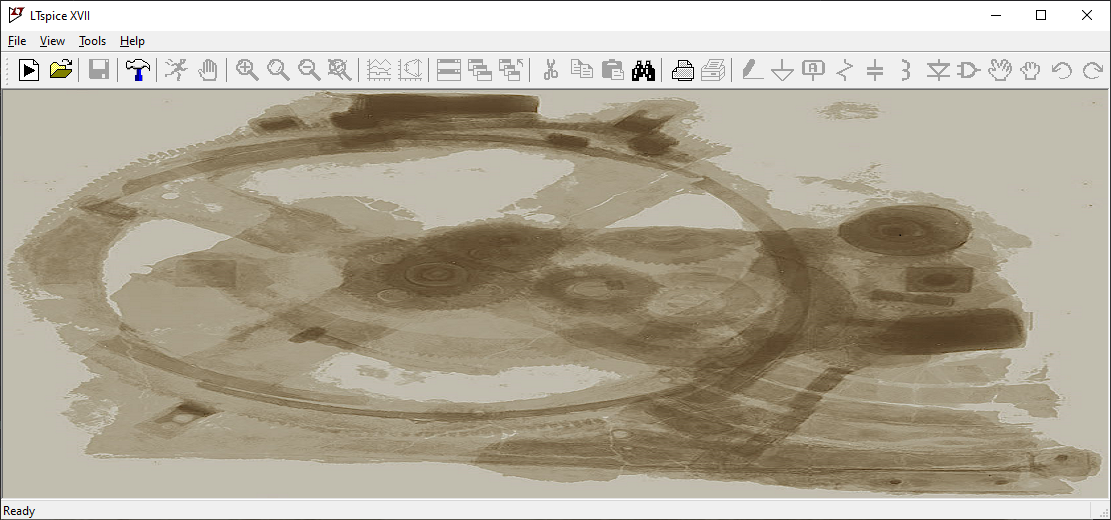
\includegraphics[scale=0.5]{IMAGENES/img2} %incluimos la imagen con una característica especial: la medida definida en centímetros e incluimos la ruta de imagen sin especificar la extensión de la imagen (solo usaremos .png y .jpg)
	\caption{Ventana de inicio de LTSpice} %La descripción de la imagen, ser concisos
	\label{img2} %La etiqueta usada para poder referenciarla desde cualquier parte del texto como se hizo con /eqref{img1}
\end{figure} %finalizamos la figura

\subsection{Creando un circuito}
Para ello nos fijamos en los íconos de la barra superior de herramientas de donde podemos agregar diferentes componentes. Podemos ir haciendo \texttt{Click} en cualquiera de ellos e ir viendo todos los componentes que podemos usar para una simulación. Se pide al lector que sea curioso con todas las opciones y vaya explorando la función de cada opción. 

\begin{figure}
	\centering
	\begin{subfigure}[b]{0.45\textwidth}
		\centering
		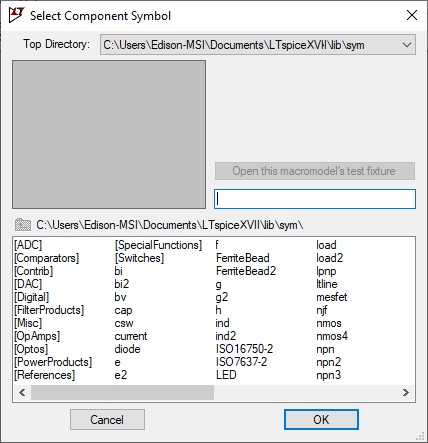
\includegraphics[scale=0.5]{IMAGENES/img3} %incluimos la imagen con una característica especial: la medida definida en centímetros e incluimos la ruta de imagen sin especificar la extensión de la imagen (solo usaremos .png y .jpg)
		\caption{Menú de componentes} %La descripción de la imagen, ser concisos
		\label{img3} %La etiqueta usada para poder referenciarla desde cualquier parte del texto como se hizo con /eqref{img1}
	\end{subfigure}
\hfill
	\begin{subfigure}[b]{0.45\textwidth}
		\centering
		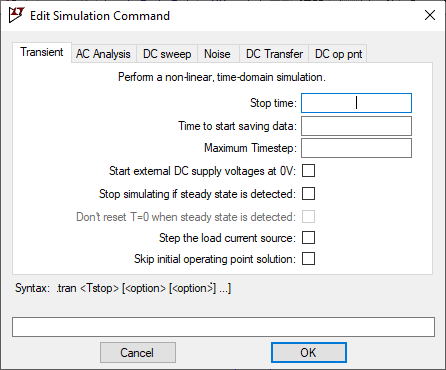
\includegraphics[scale=0.5]{IMAGENES/img5} %incluimos la imagen con una característica especial: la medida definida en centímetros e incluimos la ruta de imagen sin especificar la extensión de la imagen (solo usaremos .png y .jpg)
		\caption{Ventana para introducir comandos de Simulación.} %La descripción de la imagen, ser concisos
		\label{img5}
	\end{subfigure}
	\caption{Ventanas de opciones en LTSpice}
	\label{westminster}
\end{figure}


A continuación se presenta un circuito elelmental, en la que se tiene resistencias y una fuente de Tensión DC. Para encontrar componentes en mayor variedad, se puede hacer \texttt{Click} en el ícono que tiene forma de una compuerta AND, con lo que se mostrará un menú con mayor variedad como se muestra en la figura \eqref{img3}. Para unir las terminales de nuestros componentes, usamos la herramienta de \texttt{Cable}, que tiene el ícono de un lapiz; una vez seleccionada la herramienta, empezamos a unir cada terminal, hasta tener un circuito parecido a la figura \eqref{img4}. Para poder fijar los parámetros de los componentes de hace \texttt{Click derecho} sobre el componente. También se puede agregar texto, ya sea como comentario o como título buscando en la barra de herrramientas el correspondiente ínono, o simplemente presionando la letra \texttt{t}.

\begin{figure} %Comenzar la figura
	\centering %hacemos que la imagen en cuestion esté centrada, si guera de 5 o 6 cm, esta se vea bien
	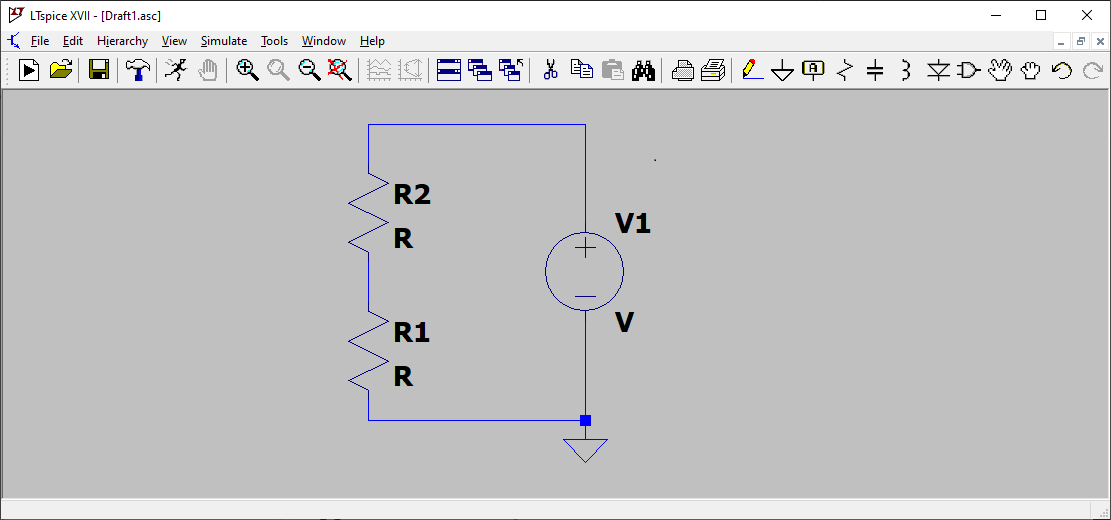
\includegraphics[scale=0.5]{IMAGENES/img4} %incluimos la imagen con una característica especial: la medida definida en centímetros e incluimos la ruta de imagen sin especificar la extensión de la imagen (solo usaremos .png y .jpg)
	\caption{Circuito resistivo elemental.} %La descripción de la imagen, ser concisos
	\label{img4} %La etiqueta usada para poder referenciarla desde cualquier parte del texto como se hizo con /eqref{img1}
\end{figure} %finalizamos la figura

Para comenzar con la simulación se busca la Herramienta \texttt{Run}, lo que generará una ventana como se muestra en la figura \eqref{img5}. podemos definir la simulación para 1 segundo (en la opción de \texttt{Stop Time}), lo que generará otra ventana. Para medir los valores de tensión por ejemplo, hacemos \texttt{Click} con la herramienta que de genera en el puntero, con el seleccionamos la una vía, y en la ventana generada, mostrará el nivel de tensión. Podemos hacer esto para otras vías de conexión, lo que generará mediciones con diferentes colores. Para generar más opciones en la ventana de medición, podemos hacer \texttt{Click} en el título del nombre de nuestro parámetro medido que generará otro cursos dándonos valores exactos. Para saber la corriente por ejemplo, hacemos \texttt{Click} sobre un componente, en cuanto se nos muestre un ícono característico de corriente en ciuanto pasemos el cursor por el componente. También es posible cambiar el nombre de nuestras vías, usando la herramienta de \texttt{Label Net}, seleccionándola, y uniéndola a una vía. 


Para cambiar en color u otras características (como hacer operaciones matemáticas para hallar potencias, u otros valores numéricos que son necesarios en circuitos más complejos) de nuestras mediciones, solo hace falta hacer doble \texttt{Click} sobre el nombre correspondiente. Para medir tensiones de un punto con respecto a otro en específico, se hace \texttt{Click} sostenido, y se suelta en otra vía, este procedimiento hará una medición que se mostrará en la ventana correspondiente. 

Algo adicional es que podemos inicializar la tensión en \texttt{0 V}, necesario para capacitores o inductores por ejemplo, para poder ver un gráfico (haciendo Zoom con su respectiva herramienta) de comportamiento real.


\section{Simulación AC de circuito de control de tono Baxandall}




Para esta simulación, abrimos un nuevo esquemático, y luego editamos el control de Comandos de simulación en la pestaña de \texttt{AC Analysis} como en la figura \eqref{img6}.

\begin{figure}
	\centering
	\begin{subfigure}[b]{0.45\textwidth}
		\centering %hacemos que la imagen en cuestion esté centrada, si guera de 5 o 6 cm, esta se vea bien
		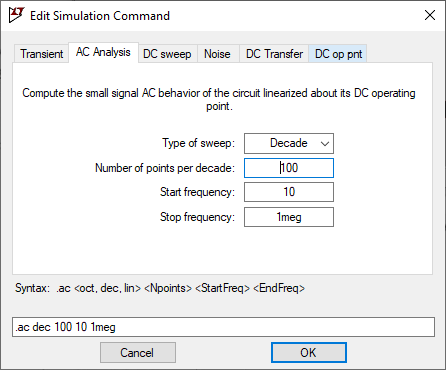
\includegraphics[scale=0.5]{IMAGENES/img6} %incluimos la imagen con una característica especial: la medida definida en centímetros e incluimos la ruta de imagen sin especificar la extensión de la imagen (solo usaremos .png y .jpg)
		\caption{Comando de Simulación del primer circuito} %La descripción de la imagen, ser concisos
		\label{img6} %La etiqueta usada para poder referenciarla desde cualquier parte del texto como se hizo con /eqref{img1}
	\end{subfigure}
	\hfill
	\begin{subfigure}[b]{0.45\textwidth}
		\centering %hacemos que la imagen en cuestion esté centrada, si guera de 5 o 6 cm, esta se vea bien
		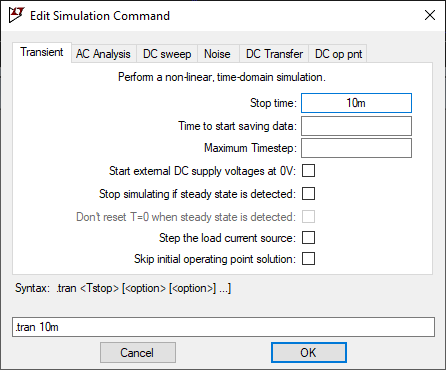
\includegraphics[scale=0.5]{IMAGENES/img9} %incluimos la imagen con una característica especial: la medida definida en centímetros e incluimos la ruta de imagen sin especificar la extensión de la imagen (solo usaremos .png y .jpg)
		\caption{Comando de Simulación de la copia.} %La descripción de la imagen, ser concisos
		\label{img9} %La etiqueta usada para poder referenciarla desde cualquier parte del texto como se hizo con /eqref{img1}
	\end{subfigure}
	\caption{Comando de Simulación.}
	\label{fuentes6y9}
\end{figure}


Después de insertar una fuente de tensión, y desplegar su opción para editar sus parámetros, se hace \texttt{Click} en la opción \texttt{Advanced} para que podamos ingresar parámentros más avanzados, como de fuente AC, fase y otros según se nececite. Para nuestra suimulación pondremos los valores como se muestran en la figura \eqref{img7}.


Nuestra simulación será un simple filtro pasa bajo, para ello incluimos una resistencia y un capacitor en serie. Para ello seteamos el resistor en \texttt{2K$\Omega$} y el capacitor en \texttt{100nF}. Para girar un componente, se debe presionar \texttt{Ctrl + R}.

Luego damos \texttt{click} en simular, y vemos nuetro gráfico al seleccionar las vías de la resistencia y el capacitor para ver la tensión. con ello veremos en la ventana de simulación en decibelios (que solo es conversión matemática) y grados.

Luego abrimos otro esquemático, donde copiamos el primer circuito (con la herramienta copiar de la barra de herramientas) y seteamos la fuente como se muestra en la figura \eqref{img8}. También editamos el control de simulación como se muestra en la figura \eqref{img9}. 

\begin{figure}
	\centering
	\begin{subfigure}[b]{0.45\textwidth}
		\centering %hacemos que la imagen en cuestion esté centrada, si guera de 5 o 6 cm, esta se vea bien
		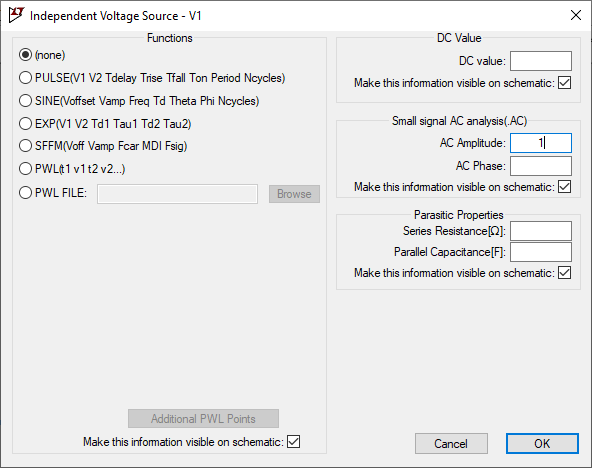
\includegraphics[scale=0.5]{IMAGENES/img7} %incluimos la imagen con una característica especial: la medida definida en centímetros e incluimos la ruta de imagen sin especificar la extensión de la imagen (solo usaremos .png y .jpg)
		\caption{Seteo del primer circuito.} %La descripción de la imagen, ser concisos
		\label{img7} %La etiqueta usada para poder referenciarla desde cualquier parte del texto como se hizo con /eqref{img1}
	\end{subfigure}
	\hfill
	\begin{subfigure}[b]{0.45\textwidth}
		\centering %hacemos que la imagen en cuestion esté centrada, si guera de 5 o 6 cm, esta se vea bien
		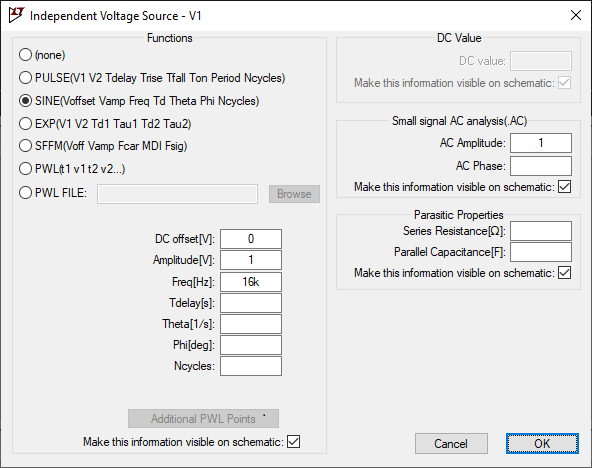
\includegraphics[scale=0.5]{IMAGENES/img8} %incluimos la imagen con una característica especial: la medida definida en centímetros e incluimos la ruta de imagen sin especificar la extensión de la imagen (solo usaremos .png y .jpg)
		\caption{Seteo para la copia del primer circuito.} %La descripción de la imagen, ser concisos
		\label{img8} %La etiqueta usada para poder referenciarla desde cualquier parte del texto como se hizo con /eqref{img1}
	\end{subfigure}
	\caption{Ventanas de seteo de la fuenute de tensión.}
	\label{fuentes7y8}
\end{figure}

Hacemos Zoom en el gráfico transitorio del segundo circuito y tendremos nuestro resultado final. Las ventanas se acomodan bien, y podemos observar nuestras simulaciones como se muestra en la figura \eqref{img10}

\begin{figure} %Comenzar la figura
	\centering %hacemos que la imagen en cuestion esté centrada, si guera de 5 o 6 cm, esta se vea bien
	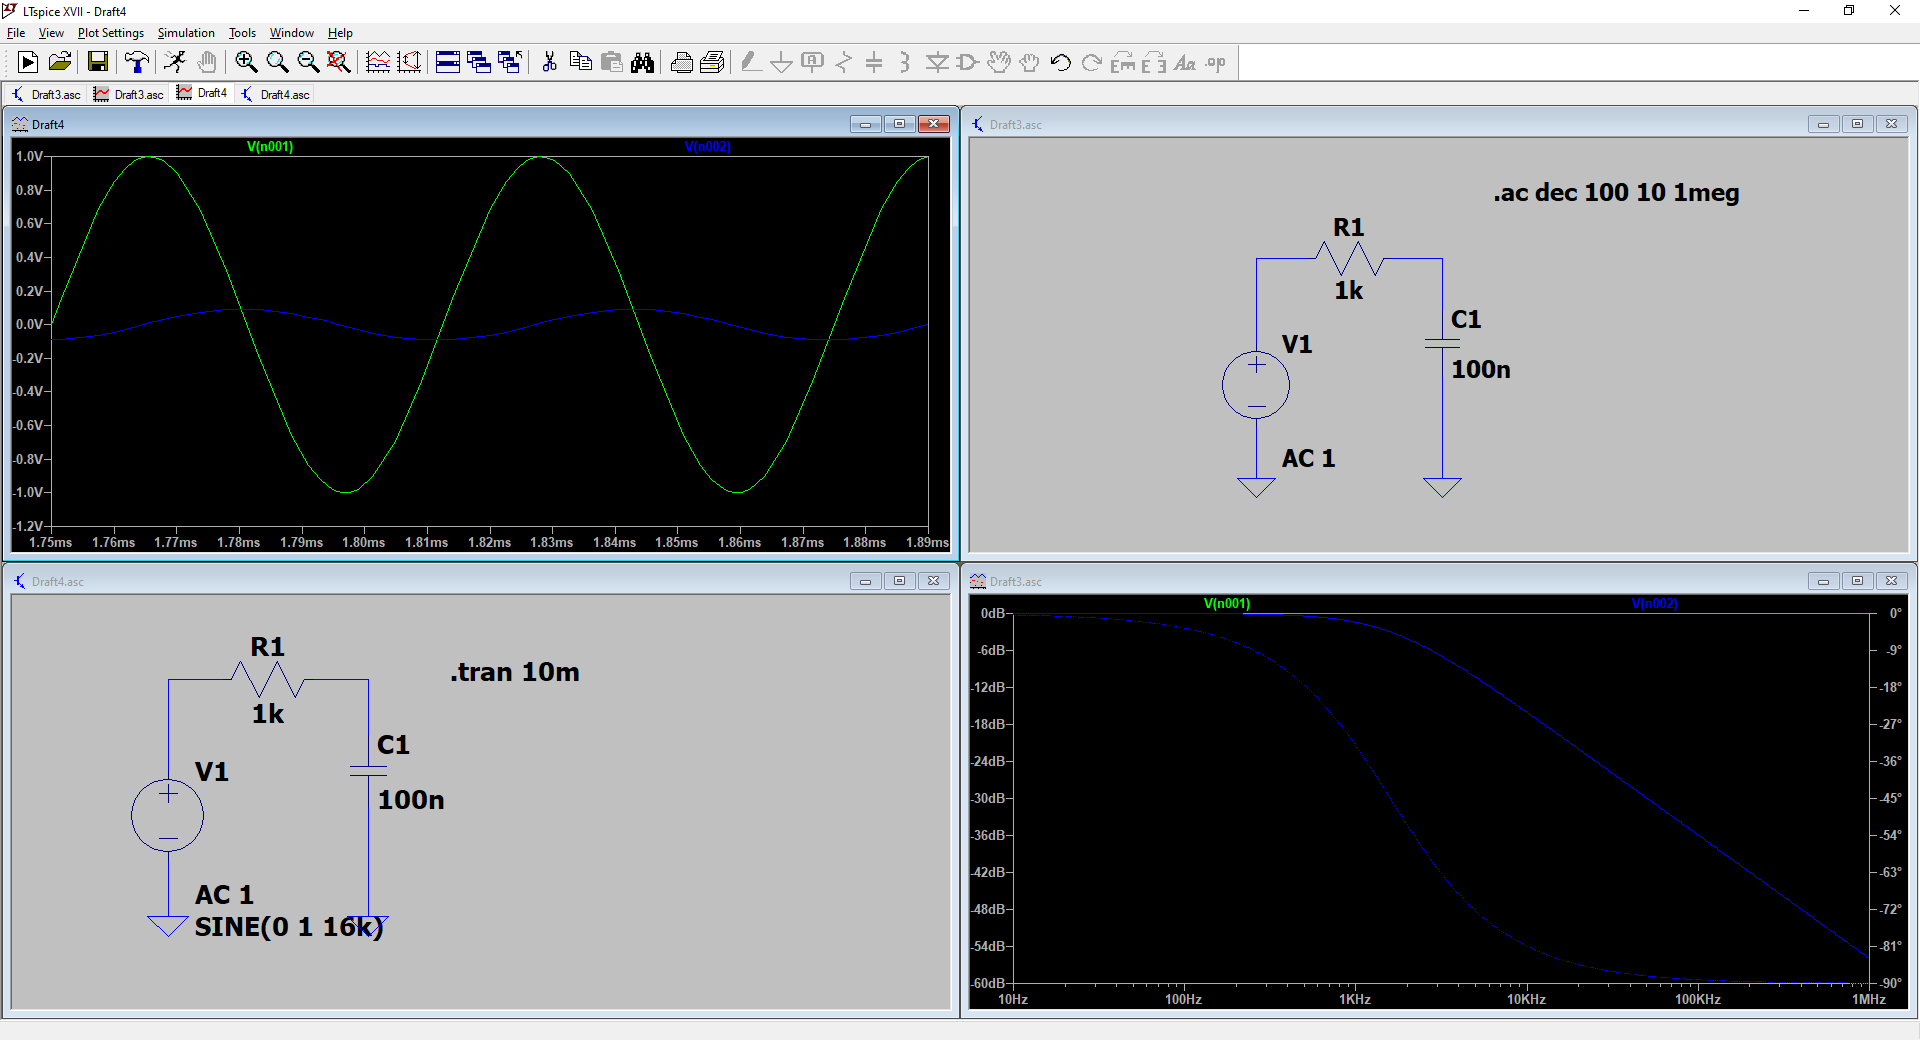
\includegraphics[scale=0.3]{IMAGENES/img10} %incluimos la imagen con una característica especial: la medida definida en centímetros e incluimos la ruta de imagen sin especificar la extensión de la imagen (solo usaremos .png y .jpg)
	\caption{Arreglo de dos circuitos con sus gráficos} %La descripción de la imagen, ser concisos
	\label{img10} %La etiqueta usada para poder referenciarla desde cualquier parte del texto como se hizo con /eqref{img1}
\end{figure} %finalizamos la figura

Ahora generamos un nuevo circuito, un circuito un poco más complejo que tenga resisten cias, capacitores y potenciómetros. Dado que LTSpice no tiene un componente llamado potenciómetro, podemos crear uno. 

Para crear un potenciómetro, después de tener una determinada disposición de resistencias, abrimos la ventana de \texttt{SPICE Directive}, o presionamos la tecla \texttt{s}. En esta ventana podemos hacer operaciones y demás a fin de simular un comportamiento del potenciómetro. Llamaremos a esta ventana el \texttt{SPICE Directive} en adelante. Como ejemplo escribimos lo que se muestra en la figura \eqref{img11} (\texttt{.param pot1 100k} y \texttt{.step param pot1dev 1 99 10} para ambos potenciometros), y tendremos los gráficos por pasos que se también se muestra en la ventana superior de la misma imagen.

Los gráficos obtenidos se pueden individualizar a solo un parámetro, ya sea tensión, corriente, fase, etc. de acuerdo a lo que se necesite.

\begin{figure} %Comenzar la figura
	\centering %hacemos que la imagen en cuestion esté centrada, si guera de 5 o 6 cm, esta se vea bien
	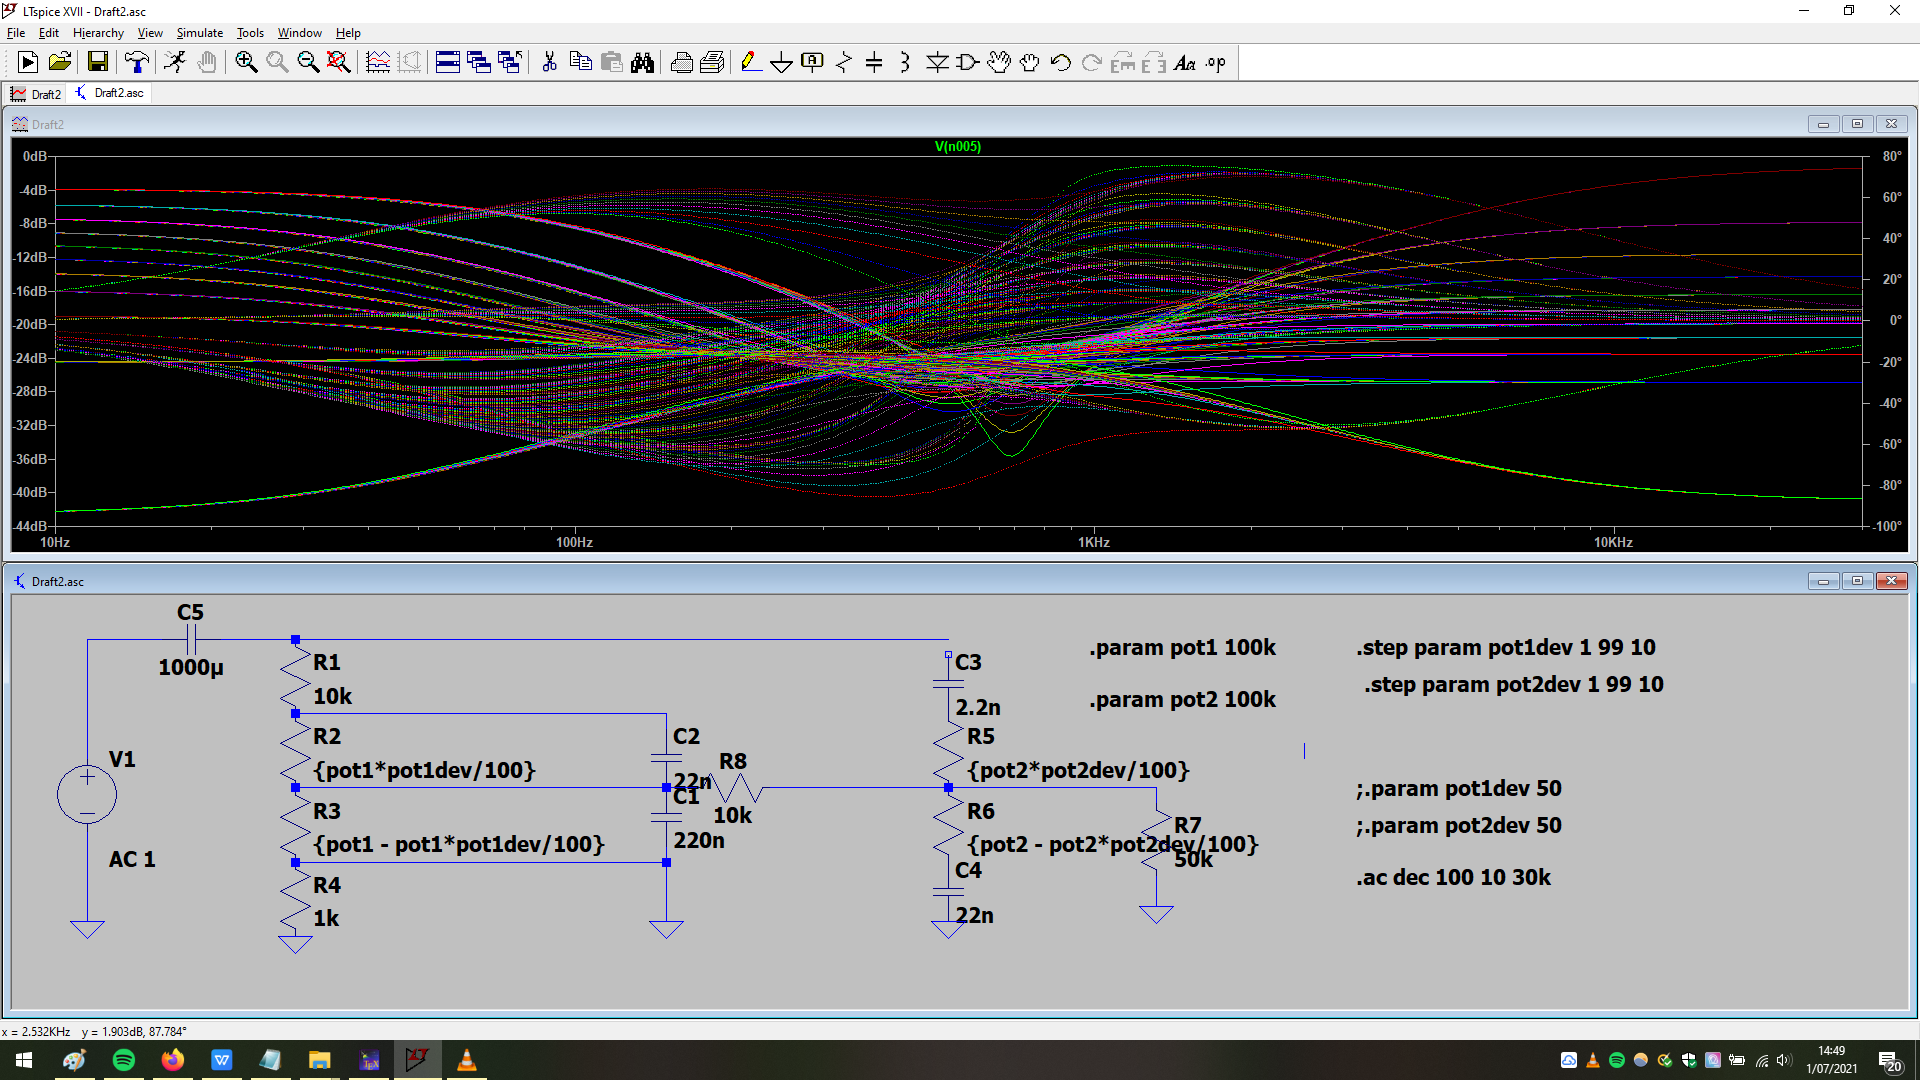
\includegraphics[scale=0.3]{IMAGENES/img11} %incluimos la imagen con una característica especial: la medida definida en centímetros e incluimos la ruta de imagen sin especificar la extensión de la imagen (solo usaremos .png y .jpg)
	\caption{Simulación final de un circuito más elaborado con graficos por pasos.} %La descripción de la imagen, ser concisos
	\label{img11} %La etiqueta usada para poder referenciarla desde cualquier parte del texto como se hizo con /eqref{img1}
\end{figure} %finalizamos la figura


\section{Directivas \texttt{.step} y \texttt{.param}}

Para poder entender mejor, podemos cerrar todo lo avanzado, y abrir un nuevo esquemático, luego dirigirnos a la pestaña de \texttt{Help} de la ventana principal, mostrándonos la ventana que se muestra en la imagen \eqref{img12}. En el explica todas las directivas que se pueden usar, con ejemplos sencillos y prácticos, pero en este capítulo explicaremos las directivas \texttt{.step} y \texttt{.param}.

\begin{figure} %Comenzar la figura
	\centering %hacemos que la imagen en cuestion esté centrada, si guera de 5 o 6 cm, esta se vea bien
	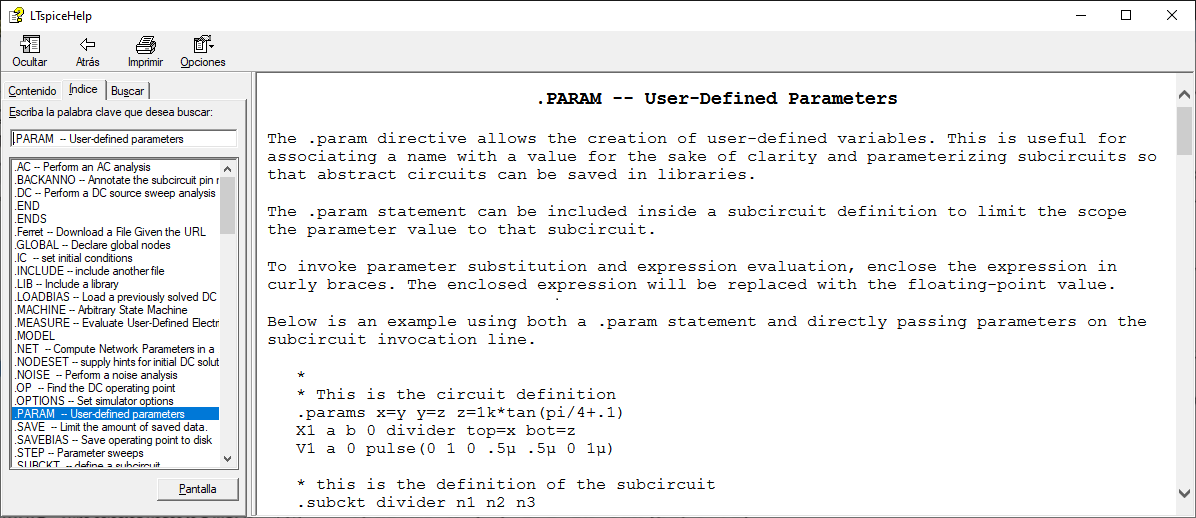
\includegraphics[scale=0.3]{IMAGENES/img12} %incluimos la imagen con una característica especial: la medida definida en centímetros e incluimos la ruta de imagen sin especificar la extensión de la imagen (solo usaremos .png y .jpg)
	\caption{Ventana de ayuda de LTSpice.} %La descripción de la imagen, ser concisos
	\label{img12} %La etiqueta usada para poder referenciarla desde cualquier parte del texto como se hizo con /eqref{img1}
\end{figure} %finalizamos la figura

Como otro ejemplo se tiene el circuito con las directivas que se indican en la figura \eqref{img13}, en el cual se muestra con todo y gráficos para las tres salidas. Una simulación parecida, pero usando la directiva \texttt{.step} se muestra en la imagen \eqref{img14} junto con su respectivo gráfico.



\begin{figure}
	\centering
	\begin{subfigure}[b]{0.45\textwidth}
		\centering %hacemos que la imagen en cuestion esté centrada, si guera de 5 o 6 cm, esta se vea bien
		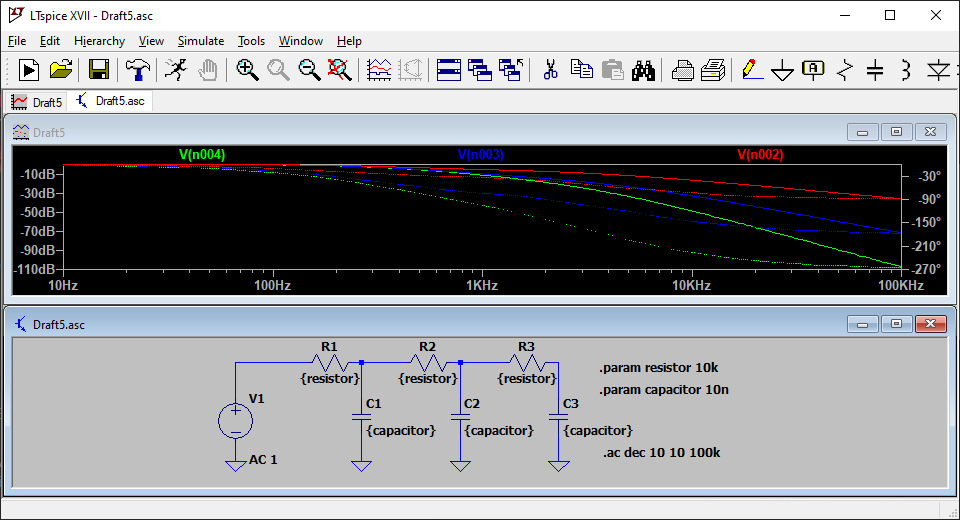
\includegraphics[scale=0.3]{IMAGENES/img13} %incluimos la imagen con una característica especial: la medida definida en centímetros e incluimos la ruta de imagen sin especificar la extensión de la imagen (solo usaremos .png y .jpg)
		\caption{Otro ejemplo con la directiva \texttt{.param}.} %La descripción de la imagen, ser concisos
		\label{img13} %La etiqueta usada para poder referenciarla desde cualquier parte del texto como se hizo con /eqref{img1}
	\end{subfigure}
	\hfill
	\begin{subfigure}[b]{0.45\textwidth}
		\centering %hacemos que la imagen en cuestion esté centrada, si guera de 5 o 6 cm, esta se vea bien
		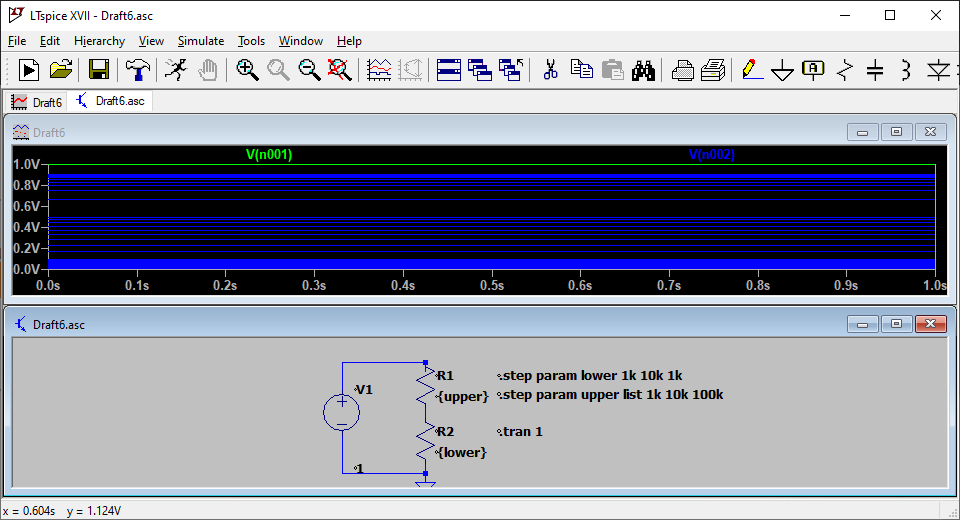
\includegraphics[scale=0.3]{IMAGENES/img14} %incluimos la imagen con una característica especial: la medida definida en centímetros e incluimos la ruta de imagen sin especificar la extensión de la imagen (solo usaremos .png y .jpg)
		\caption{Otro ejemplo con la directiva \texttt{.step}.} %La descripción de la imagen, ser concisos
		\label{img14} %La etiqueta usada para poder referenciarla desde cualquier parte del texto como se hizo con /eqref{img1}
	\end{subfigure}
	\caption{Uso de directivas.}
	\label{fuentes13y14}
\end{figure}

\section{Importar Librerías y modelos de componentes}

Todos tuvimos en algún momento la necesidad de usar un componente específico, y el no encontrarlo entre el catálogo de dispositivos que se ofrecen en determinado simulador, es un grán problema porque la simulación no se podría hacer de manera correcta. 

Para poder solucionar ese problema, LTSpice permite la importación de librerías y modelos de otros componentes, y los pasos para hacerlo se muestran a continuación.

\subsection{Buscar en un Navegador}

Para este ejemplo buscamos el modelo de un diodo, el diodo \texttt{1n4004} para ser más específicos. Lo buscamo como \texttt{1n4004 spice model}. En nuestro ejemplo entramos al modelo de la página \url{https://www.onsemi.com} y hacemos \texttt{click} en donde señala \texttt{Simulation Model > Spice Model} lo que hará que se descargue un archivo de extensión \texttt{.LIB}. 

\begin{figure} %Comenzar la figura
	\centering %hacemos que la imagen en cuestion esté centrada, si guera de 5 o 6 cm, esta se vea bien
	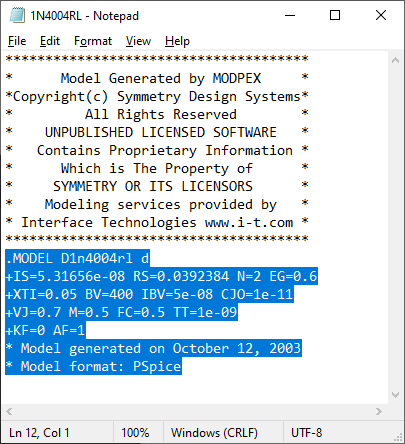
\includegraphics[scale=0.4]{IMAGENES/img15} %incluimos la imagen con una característica especial: la medida definida en centímetros e incluimos la ruta de imagen sin especificar la extensión de la imagen (solo usaremos .png y .jpg)
	\caption{Modelo Spice del diodo \texttt{1n4004}.} %La descripción de la imagen, ser concisos
	\label{img15} %La etiqueta usada para poder referenciarla desde cualquier parte del texto como se hizo con /eqref{img1}
\end{figure} %finalizamos la figura

\subsection{Edición en LTSpice}

Lo siguiente es abrir el archivo con un editor de texto, puede ser Notepad de Windows con lo que tendremos la información de la librería como se muestra en la figura \eqref{img15}. Luego copiamos tan solo el modelo para crear una nueva directiva, presionando la tecla \texttt{S}, y la colocamos en la ventana del esquemático, como se muestra en la figura \eqref{img16}.

\begin{figure} %Comenzar la figura
	\centering %hacemos que la imagen en cuestion esté centrada, si guera de 5 o 6 cm, esta se vea bien
	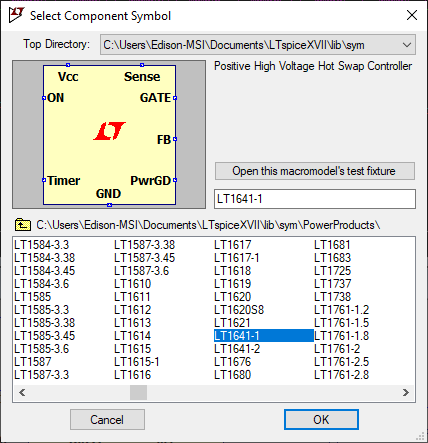
\includegraphics[scale=0.4]{IMAGENES/img16} %incluimos la imagen con una característica especial: la medida definida en centímetros e incluimos la ruta de imagen sin especificar la extensión de la imagen (solo usaremos .png y .jpg)
	\caption{Modelo Spice del diodo \texttt{1n4004} en un circuito elemental.} %La descripción de la imagen, ser concisos
	\label{img16} %La etiqueta usada para poder referenciarla desde cualquier parte del texto como se hizo con /eqref{img1}
\end{figure} %finalizamos la figura

Para enlazarlo al diodo ya exportado en el esquemático, cambiamos el nombre del diodo como ya sabemos por el nombre del modelo que escribimos en la directiva, que en nuestro caso sería \texttt{D1n4004rl}.

Otra forma de incluir una librería, es viendo lo que describe \texttt{.include}, información que podemos encontrar en la pestaña de \texttt{Help > LTspiceHelp}. En el dice que podemos incluir nuestro fichero \texttt{.LIB} en un directorio, el cual por defecto podría ser el que muestra en el texto, o podría ser el que hayamos elegido cuando instalamos \texttt{LTSpice}. Po lo general debemos copiar el fichero a \texttt{.../lib/sub}. Luego, en la simulación, copiamos el nombre del fichero con todo y extensión y la agregamos con la ventana de \texttt{SPICE Directive} comenzando con \texttt{.inc D1n4004rl.LIB} por ejemplo. Luego simulamos y obtendremos el mismo resultado. También se puede cambiar el nombre del diodo desde el código fuente, yendonos a la carpeta de \texttt{.../lib/cmp} donde podemos seleccionar el fichero de diodos por ejemplo, y buscar el diodo que queremos modificar. Para comprobar su funcionamiento, hacemos la prueba de simulación y tendremos un modo más de edición de parámetros de un dispositivo.

Siguiendo este mismo procedimiento, podemos agregar multiples dispositivos, de diferentes páginas tan solo fijándonos que el modelo matemático que buscamos está en \texttt{Spice Model}. Al final, viendo el código fuente de las librerias que se están usando, podemos crear nuestros propios dispositivos con parámetros específicos que necesitamos para una simulación. Podemos crear modelos a partir de componentes ya existentes. Las posibilidades son muy diversas, y el alcance de simulación solo estará limitada por las habilidades de la persona a cargo.

\section{Ejemplos y simulaciones para divertirse}

LTSpice nos da la opción de analizar una gran variedad de circuitos ya diseñados, a fin de que podamos variar sus parámetros y ver el comportamiento en la ventana de gráficos usando diferentes unidades. Para ello no hace falta más explicación, ya depende del grado de curiosidad del lector para poder pasar mucho tiempo analizando, simulando, variando parámetros viendo el comportamiento en diferentes condiciones de todos los circuitos que se muestran. A continuación se presentran dos formas para poder jugar con estos circuitos.

\subsection{Circuitos a partir del catálogo de componentes}

Lo primero que hacemos es ir al ícono para elegir componentes, y ya en la ventana elegir un componente de nuestra preferencia, desde resistencias hasta compejas fuentes de tensión o amplificadores muy elaborados. Lo que se mostrará es algo asó como la figura \eqref{img17}, donde una vez que hayamos seleccionado el componente de nuestra preferencia, le daremos click en la opción de \texttt{Open this macromodel's test fixture}. Luego solo queda jugar con los parámetros y ver el comportamiento en el monitor de gráficos.

\begin{figure} %Comenzar la figura
	\centering %hacemos que la imagen en cuestion esté centrada, si guera de 5 o 6 cm, esta se vea bien
	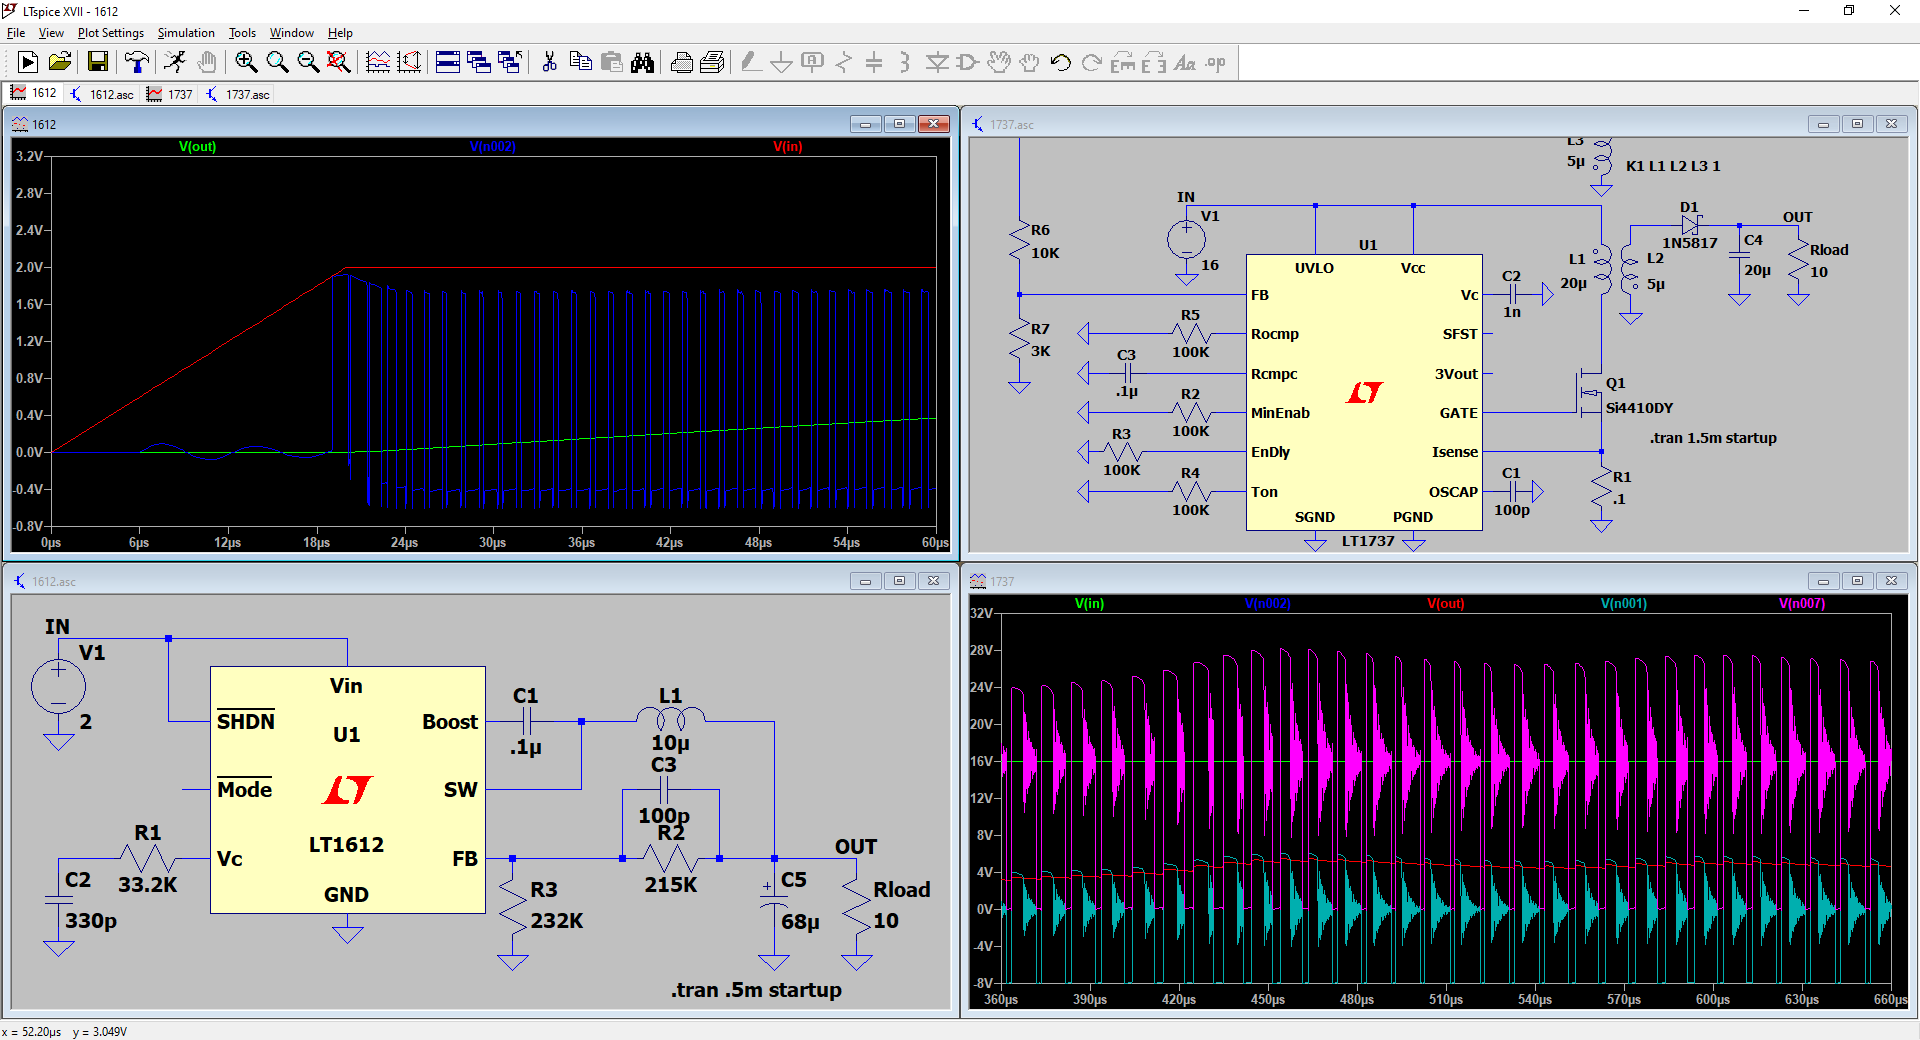
\includegraphics[scale=0.3]{IMAGENES/img17} %incluimos la imagen con una característica especial: la medida definida en centímetros e incluimos la ruta de imagen sin especificar la extensión de la imagen (solo usaremos .png y .jpg)
	\caption{Simulaciones con circuitos prediseñados para poder ver el comportamiento del componente de preferencia.} %La descripción de la imagen, ser concisos
	\label{img17} %La etiqueta usada para poder referenciarla desde cualquier parte del texto como se hizo con /eqref{img1}
\end{figure} %finalizamos la figura

\subsection{Abriendo diseños desde el directorio}

Para esllo nos vamos a la pestaña de \texttt{Open} y nos dirigimos a la carpeta \texttt{.../LTspiceXVII/examples}, donde tendremos \texttt{jigs} y la otra carpeta \texttt{Educational}. ambas carpetas guardan una gran variedad de circuitos que podemos ir explorando a fin de afianzar nuestros conocimientos de electrónica y ver comportamientos de circuitos reales, con funcionamiento comercial y de investigación. En la imagen \eqref{img18} se muestra unos ejemplos con los parámetros que podemos ver en el catálogo de circuitos presentados.

\begin{figure} %Comenzar la figura
	\centering %hacemos que la imagen en cuestion esté centrada, si guera de 5 o 6 cm, esta se vea bien
	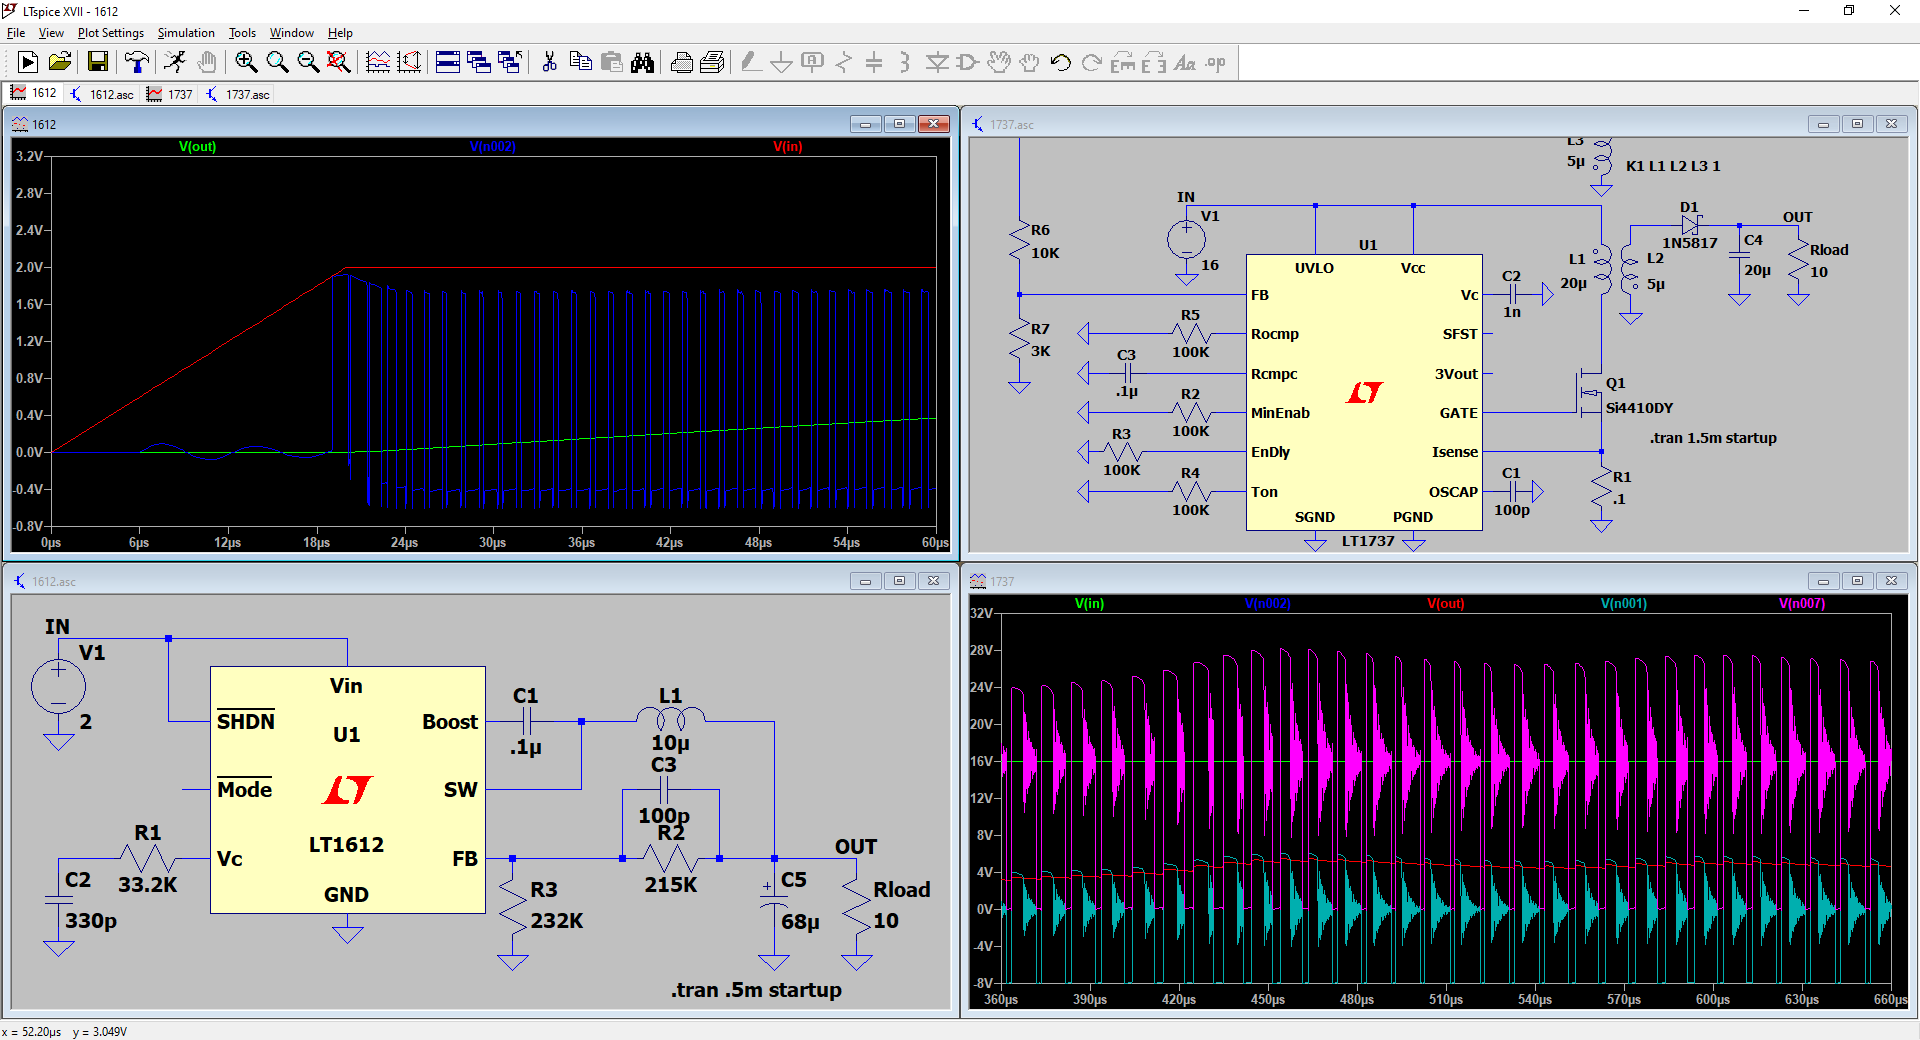
\includegraphics[scale=0.3]{IMAGENES/img17} %incluimos la imagen con una característica especial: la medida definida en centímetros e incluimos la ruta de imagen sin especificar la extensión de la imagen (solo usaremos .png y .jpg)
	\caption{Circuitos completos y funcionales listos para su uso.} %La descripción de la imagen, ser concisos
	\label{img18} %La etiqueta usada para poder referenciarla desde cualquier parte del texto como se hizo con /eqref{img1}
\end{figure} %finalizamos la figura

\section{Conceptos de FFT y declaración \texttt{.four}}

Una manera muy sencilla de ver la FFT de una fuente sencilla que se crea como en la imagen \eqref{img19} es haciendo \texttt{click} derecho en el monitor de gráficos y luego ir a \texttt{View > FFT}, luego seleccionamos nuestra fuente y podremos ver la FFT. 

\begin{figure} %Comenzar la figura
	\centering %hacemos que la imagen en cuestion esté centrada, si guera de 5 o 6 cm, esta se vea bien
	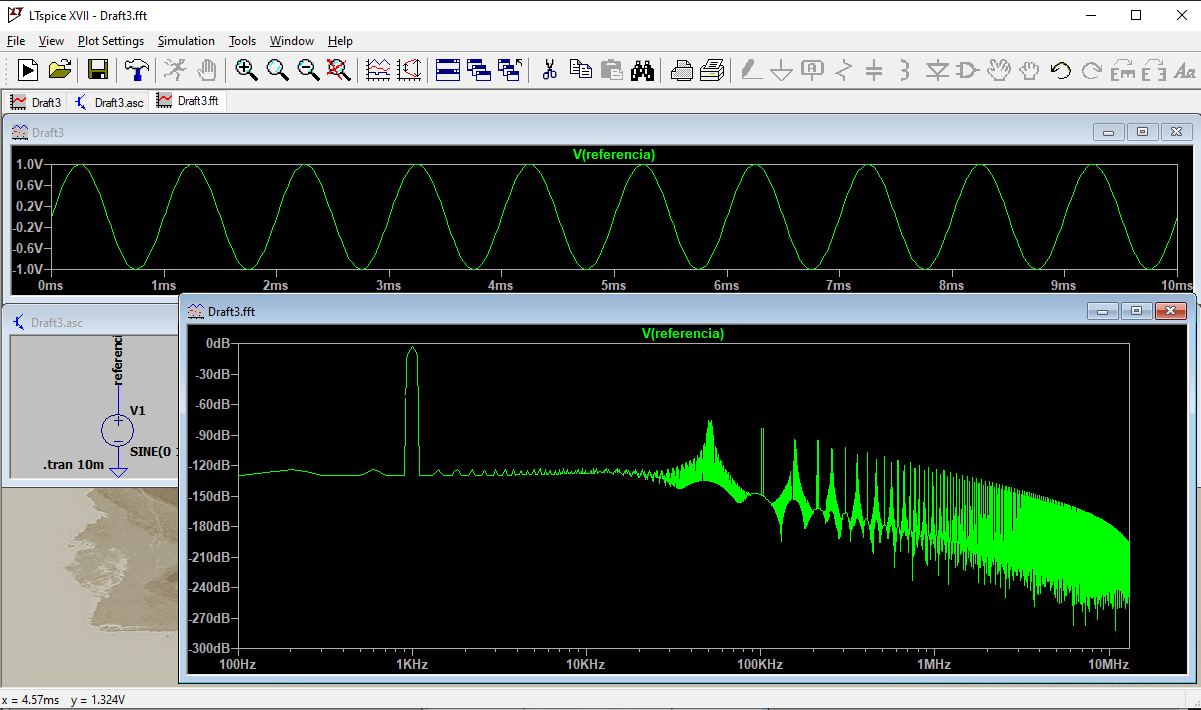
\includegraphics[scale=0.3]{IMAGENES/img19} %incluimos la imagen con una característica especial: la medida definida en centímetros e incluimos la ruta de imagen sin especificar la extensión de la imagen (solo usaremos .png y .jpg)
	\caption{Vista de FFT para una fuente de 1KHz con amplitud de 1V.} %La descripción de la imagen, ser concisos
	\label{img19} %La etiqueta usada para poder referenciarla desde cualquier parte del texto como se hizo con /eqref{img1}
\end{figure} %finalizamos la figura

Se piuede ver mucho ruido, y por supuesto, lo que esperábamos, la muestra en \texttt{1KHz}.

Para mejorar nuestra salida, vamos a la pestaña de ayuda, para buscar \texttt{.options}. En el buscamos \texttt{numdgt} que nos dará doble precisión según lo descrito. Luego la agregamos a nuestra simulación como lo hacíamos con \texttt{.step} por ejemplo. agregamos \texttt{.options numdgt = 7}. Lo siguiente que buscamos en \texttt{.options} es \texttt{plotwinzise} que nla usamos para comprimir mejor nuestros datos. Agregamos \texttt{.options plotwinsize = 0}. Esto nos dará una vista de FFT más limpia que el inicial, como se muestra en la figura \eqref{img20}

\begin{figure} %Comenzar la figura
	\centering %hacemos que la imagen en cuestion esté centrada, si guera de 5 o 6 cm, esta se vea bien
	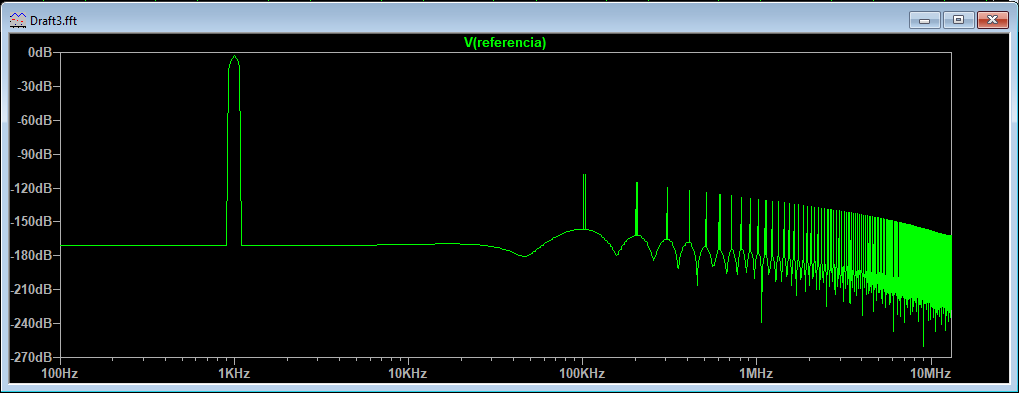
\includegraphics[scale=0.4]{IMAGENES/img20} %incluimos la imagen con una característica especial: la medida definida en centímetros e incluimos la ruta de imagen sin especificar la extensión de la imagen (solo usaremos .png y .jpg)
	\caption{Vista de FFT para una fuente de 1KHz con amplitud de 1V usando \texttt{.options numdgt = 7} y \texttt{.options plotwinsize = 0}.} %La descripción de la imagen, ser concisos
	\label{img20} %La etiqueta usada para poder referenciarla desde cualquier parte del texto como se hizo con /eqref{img1}
\end{figure} %finalizamos la figura

El ruido que aún se ve es debido a las muestras que se toman en la simulación, por lo que podemos variar el \texttt{Maximum Timestep} en nuestro comando de simulación con \texttt{100n} segundos por ejemplo. Haciendo pruebas, y viendo que la computadora se tarda un poco en generar las muestras, se probó con un \texttt{Timestep} de \texttt{1n} segundo, y el resultado es lo que se muestra en la imagen \eqref{img21}. Lo que también se puede hacer es aumentar el \texttt{Stop Time} del panel de simulación para generar aparente limpieza en el resultado.

\begin{figure} %Comenzar la figura
	\centering %hacemos que la imagen en cuestion esté centrada, si guera de 5 o 6 cm, esta se vea bien
	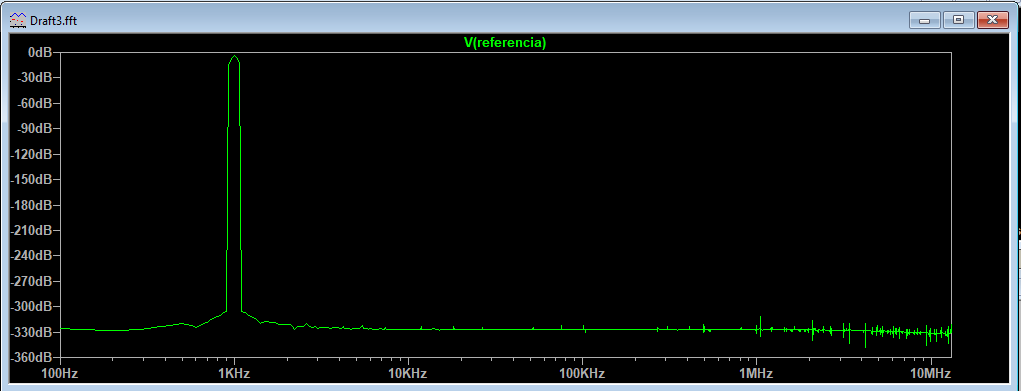
\includegraphics[scale=0.4]{IMAGENES/img21} %incluimos la imagen con una característica especial: la medida definida en centímetros e incluimos la ruta de imagen sin especificar la extensión de la imagen (solo usaremos .png y .jpg)
	\caption{Vista de FFT para una fuente de 1KHz con amplitud de 1V usando \texttt{.options numdgt = 7} y \texttt{.options plotwinsize = 0}. para un \texttt{Timestep} de \texttt{1n} segundo.} %La descripción de la imagen, ser concisos
	\label{img21} %La etiqueta usada para poder referenciarla desde cualquier parte del texto como se hizo con /eqref{img1}
\end{figure} %finalizamos la figura

También se puede usar la declaración \texttt{.four}, y la podemos ver, como es de costumbre, desde \texttt{LTspiceHelp}. En el podemos ver que es posible agregar la frecuencia, el n;umero de armónicos, de periodos y lo demás, en el orden que señala su descripción. Para el ejemplo agregamos \texttt{.four 1000 10 100 v(referencia)}. Luego vemos en la pestaña de \texttt{View > SPICE Error Log}, donde podremos ver la data como se muestra en la figura \eqref{img22}

\begin{figure} %Comenzar la figura
	\centering %hacemos que la imagen en cuestion esté centrada, si guera de 5 o 6 cm, esta se vea bien
	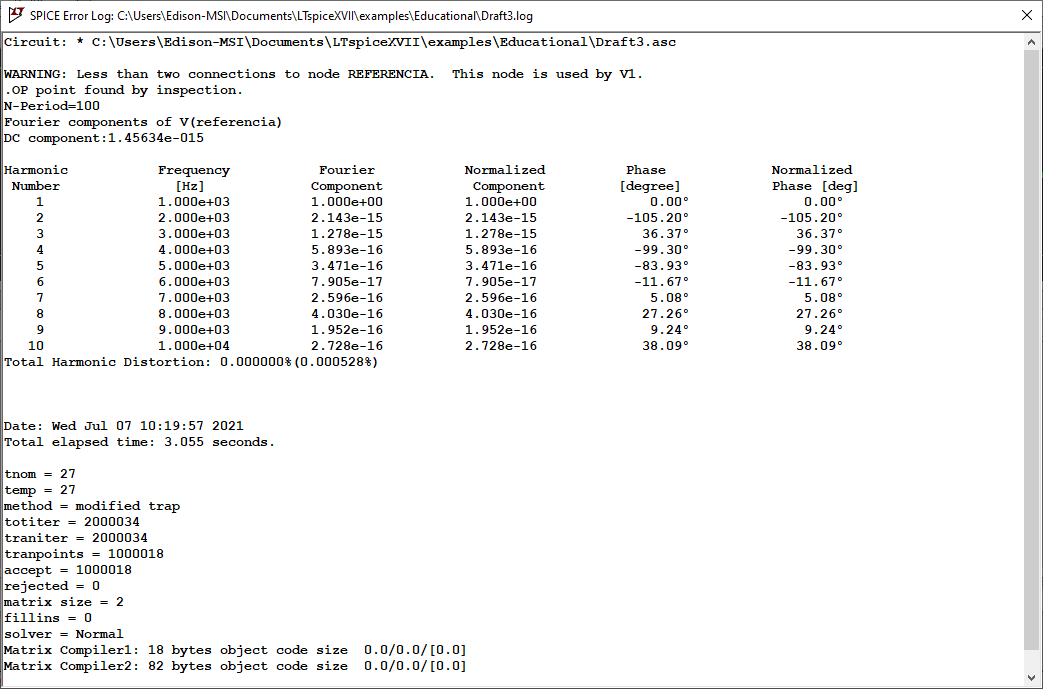
\includegraphics[scale=0.4]{IMAGENES/img22} %incluimos la imagen con una característica especial: la medida definida en centímetros e incluimos la ruta de imagen sin especificar la extensión de la imagen (solo usaremos .png y .jpg)
	\caption{Datos mostrados de la FFT.} %La descripción de la imagen, ser concisos
	\label{img22} %La etiqueta usada para poder referenciarla desde cualquier parte del texto como se hizo con /eqref{img1}
\end{figure} %finalizamos la figura

Ahora creamos un circuito sencillo, introducimos valores (ver figura \eqref{img24}) y simulamos con lo ya aprendido. Vemos el error de armónicos (figura \eqref{img23}) y veremos el gráfico final de la figura \eqref{img24} mucho más aceptable, y con menos ruido que en un inicio.

\begin{figure} %Comenzar la figura
	\centering %hacemos que la imagen en cuestion esté centrada, si guera de 5 o 6 cm, esta se vea bien
	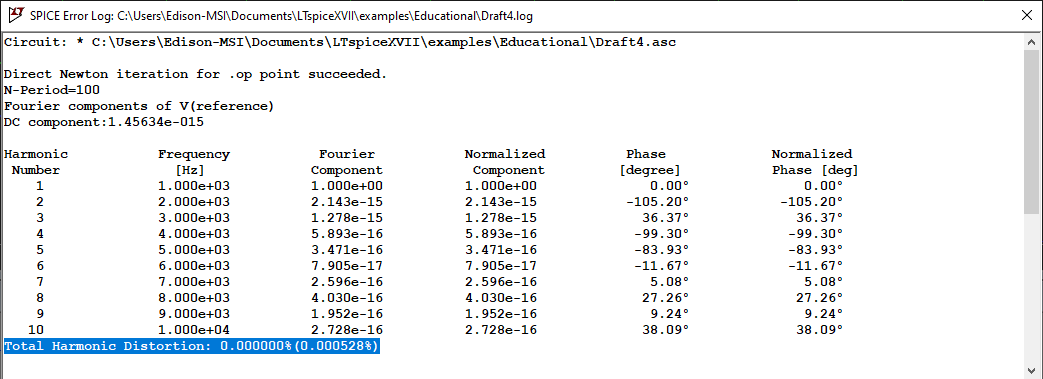
\includegraphics[scale=0.4]{IMAGENES/img23} %incluimos la imagen con una característica especial: la medida definida en centímetros e incluimos la ruta de imagen sin especificar la extensión de la imagen (solo usaremos .png y .jpg)
	\caption{Datos mostrados de la FFT.} %La descripción de la imagen, ser concisos
	\label{img23} %La etiqueta usada para poder referenciarla desde cualquier parte del texto como se hizo con /eqref{img1}
\end{figure} %finalizamos la figura

\begin{figure} %Comenzar la figura
	\centering %hacemos que la imagen en cuestion esté centrada, si guera de 5 o 6 cm, esta se vea bien
	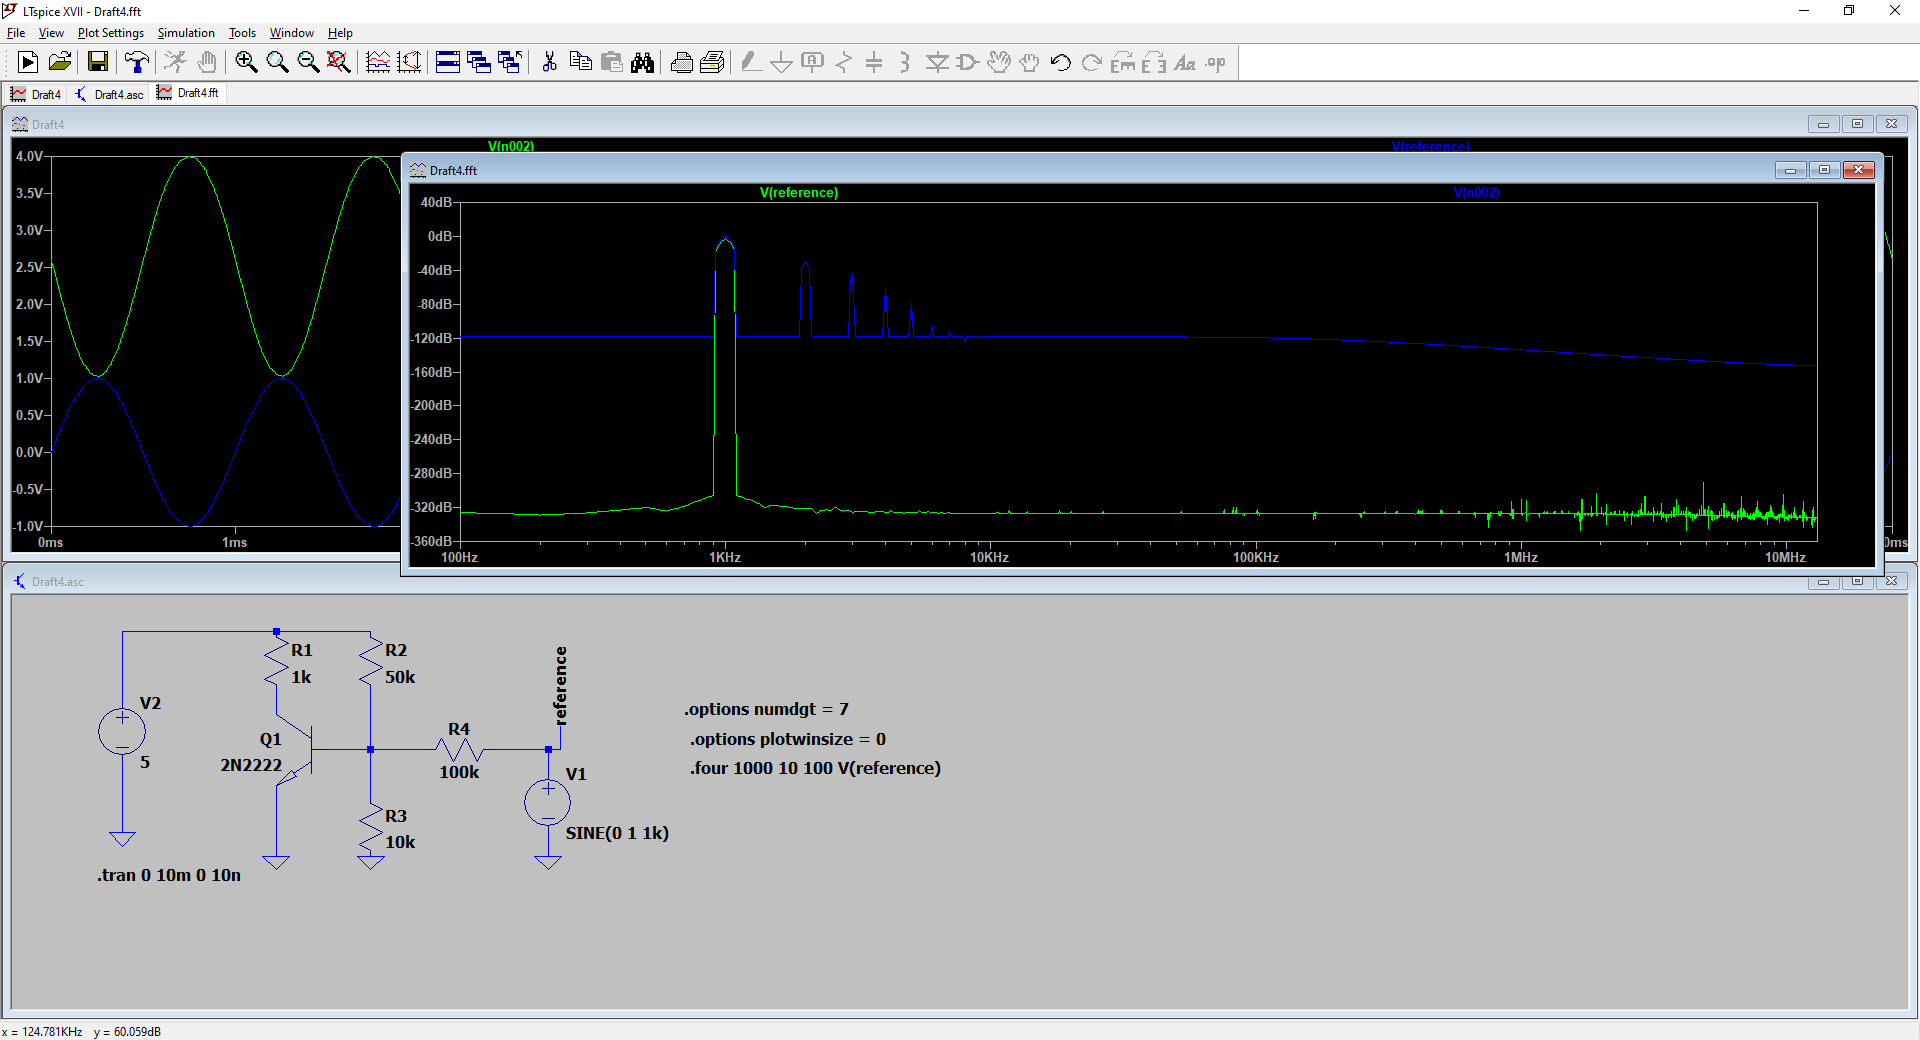
\includegraphics[scale=0.3]{IMAGENES/img24} %incluimos la imagen con una característica especial: la medida definida en centímetros e incluimos la ruta de imagen sin especificar la extensión de la imagen (solo usaremos .png y .jpg)
	\caption{Resultado con el circuito sencillo que muestra la FFT.} %La descripción de la imagen, ser concisos
	\label{img24} %La etiqueta usada para poder referenciarla desde cualquier parte del texto como se hizo con /eqref{img1}
\end{figure} %finalizamos la figura

\section{Fuentes de Tension y Corriente dependientes.}

Vamos a \texttt{LTSpiceHelp} para ver \texttt{.E} que es nuestra fuente de voltaje dependiente con lo que ya podemos ver toda su descripción ahí. para agregar el componente en nuestro esquemático, agregamos \texttt{e} de nuestro catálogo de componentes y vamos armando un circuito sencillo como se muestra en la figura \eqref{img25} las diferentes configuraciones y sus usos se describen en la pestaña de \texttt{LTspiceHelp}. Podemos ver las fuentes \texttt{.e, .g, .h, .f o B.} para usar formulas matemáticas para manejar fuentes dependientes con modelos matemáticos. esto puede ser util para modelar transistores como fuentes dependientes por ejemplo.

\begin{figure} %Comenzar la figura
	\centering %hacemos que la imagen en cuestion esté centrada, si guera de 5 o 6 cm, esta se vea bien
	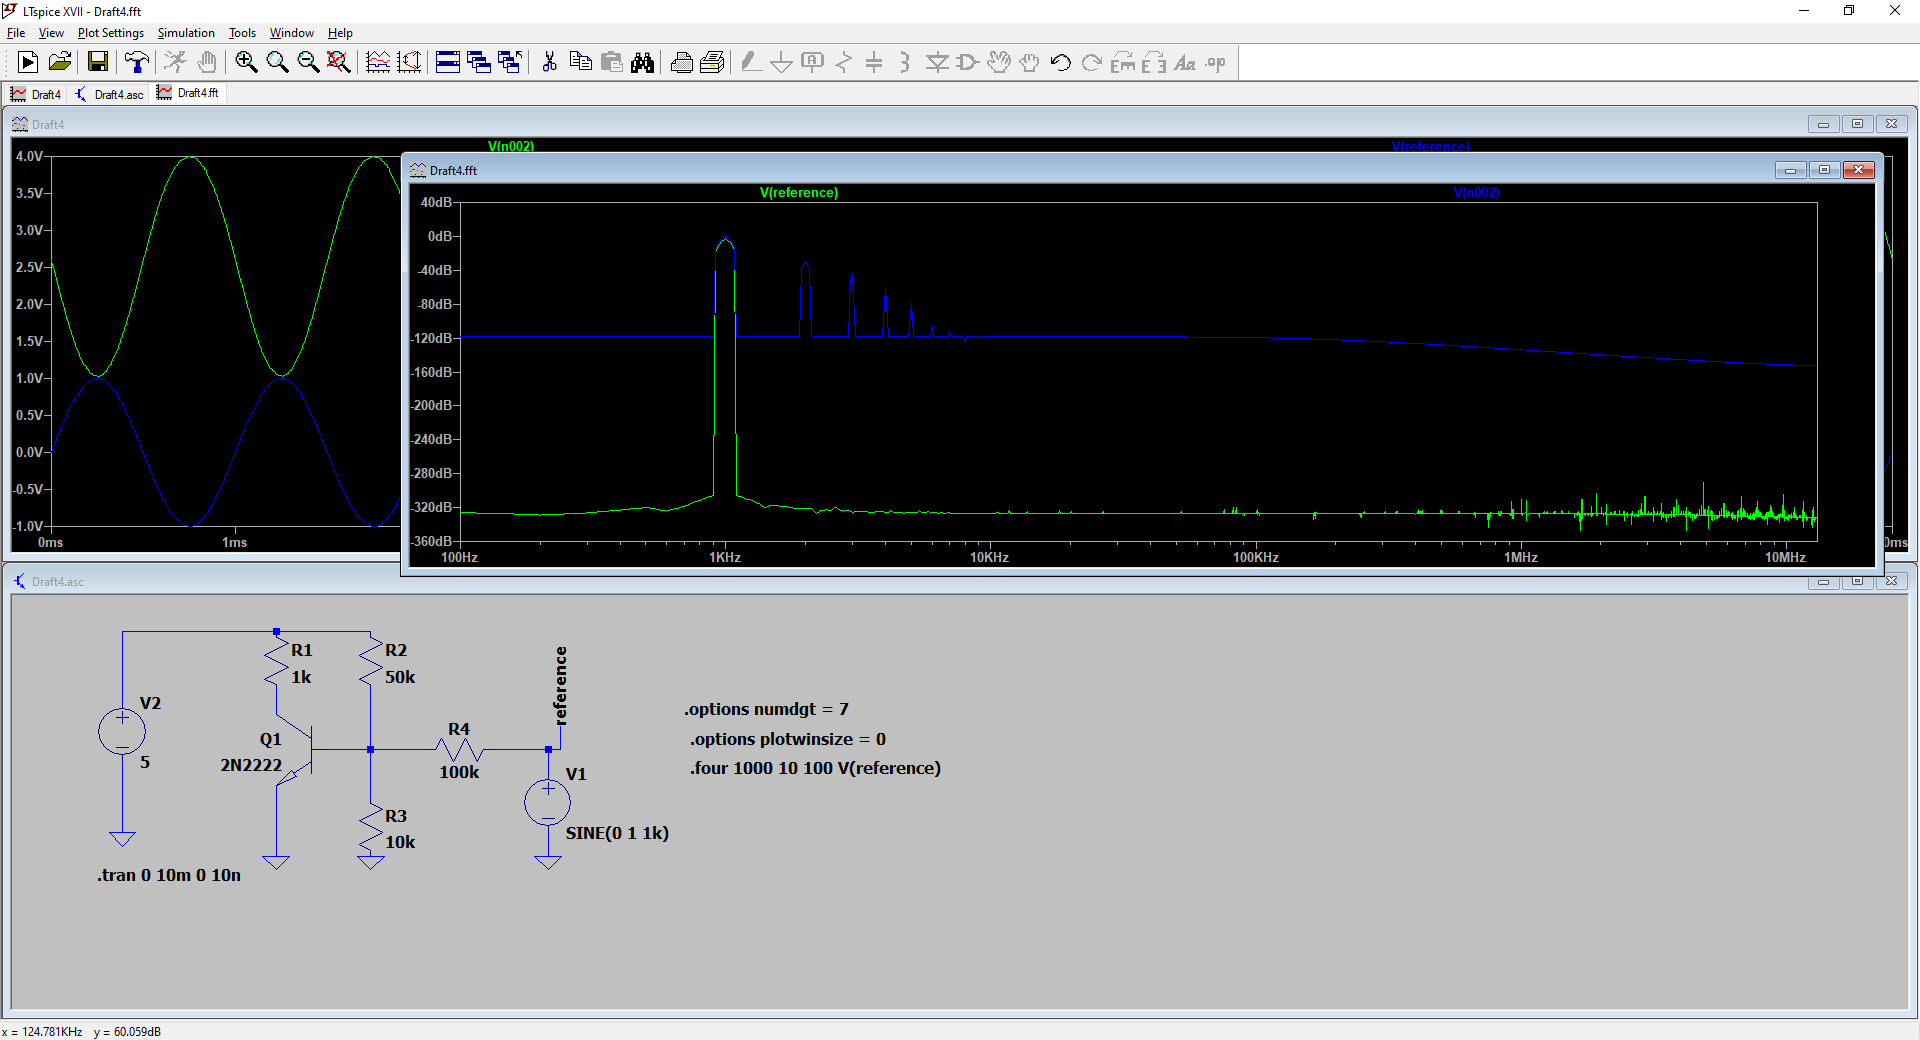
\includegraphics[scale=0.3]{IMAGENES/img24} %incluimos la imagen con una característica especial: la medida definida en centímetros e incluimos la ruta de imagen sin especificar la extensión de la imagen (solo usaremos .png y .jpg)
	\caption{Fuente de tensión y corriente dependiente.} %La descripción de la imagen, ser concisos
	\label{img25} %La etiqueta usada para poder referenciarla desde cualquier parte del texto como se hizo con /eqref{img1}
\end{figure} %finalizamos la figura 

	%%%%%%%%%%%%%%%%%%%%%%%%%%%%%%%%%%%%%%%%%%%%%%%
	%%%%%
	%%%%%   BIBLIOGRAFÍA    %%%%%%%%%%%%%%%%%%%%%% No tenemos :'v sad
	%%%%%
	%%%%%%%%%%%%%%%%%%%%%%%%%%%%%%%%%%%%%%%%%%%%%%%
	
	
	
%	\bibliographystyle{ieeetr}
%	\bibliography{bibliografia}
	
\end{document}

